\section{Equilibrium}
When the simulation starts, the system is far from equilibrium. [[why?]] To push the system towards equilibrium, the particle velocities are rescaled with scaling factor $\lambda$:
\begin{gather}\label{eq:rescale}
    \lambda=\sqrt{\frac{(N-1)3k_BT_D}{\sum_{i=1}^{N} mv_i^{2}}}.
\end{gather} After each rescaling a jump in the system temperature $T$ towards the desired temperature $T_d$ occurs. This can be seen in figure \ref{fig:temp}, where the system temperature vs time is plotted when the system is still in the equilibration phase. Here, rescaled is performed every 40 time steps.
\begin{Figure}
 \centering
 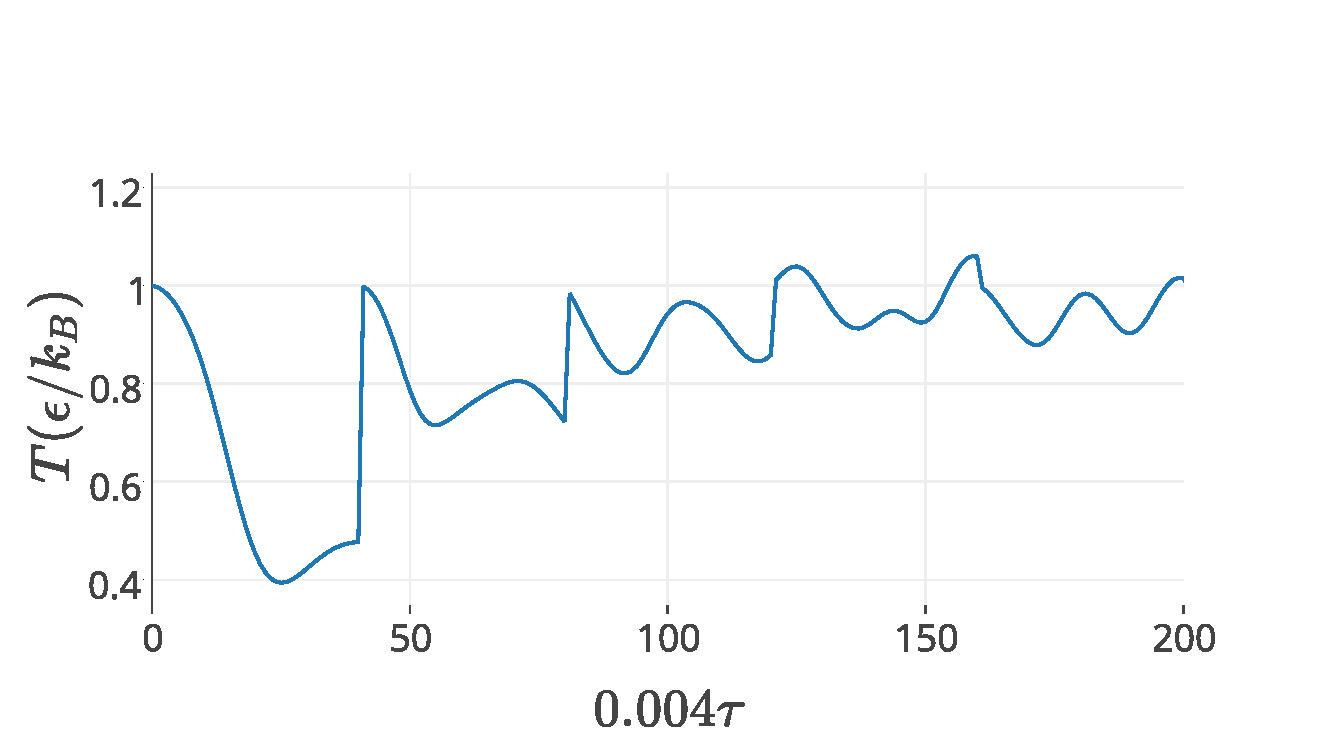
\includegraphics[width=1\linewidth]{equilibration.eps}
 \captionof{figure}{Temperature in equilibration phase. The effects of rescaling can be seen as discontinuities in $T$, every 40 time steps.}\label{fig:temp}
\end{Figure}
% A simulation for 108 particles was run, figure %\ref{fig:instant_temp}
% shows the instantaneous temperature as a function of time steps. The desired temperature was set to 300~K. The temperature fluctuates a lot at the start of the simulation, since the system is far from equilibrium. After around 1000 time steps the system appears to reach equilibrium and the temperature fluctuates around $T_D$. During the equilibration phase the particle velocity is rescaled at intervals of 200 time steps, with the rescaling factor from Eq. \ref{eq:rescale}. Now that the system is in equilibrium, physical quantities can be extracted from the simulation.